\documentclass{thesis}
% \geometry{showframe}
\usepackage{subfiles}

\addbibresource{references.bib}

\begin{document}
	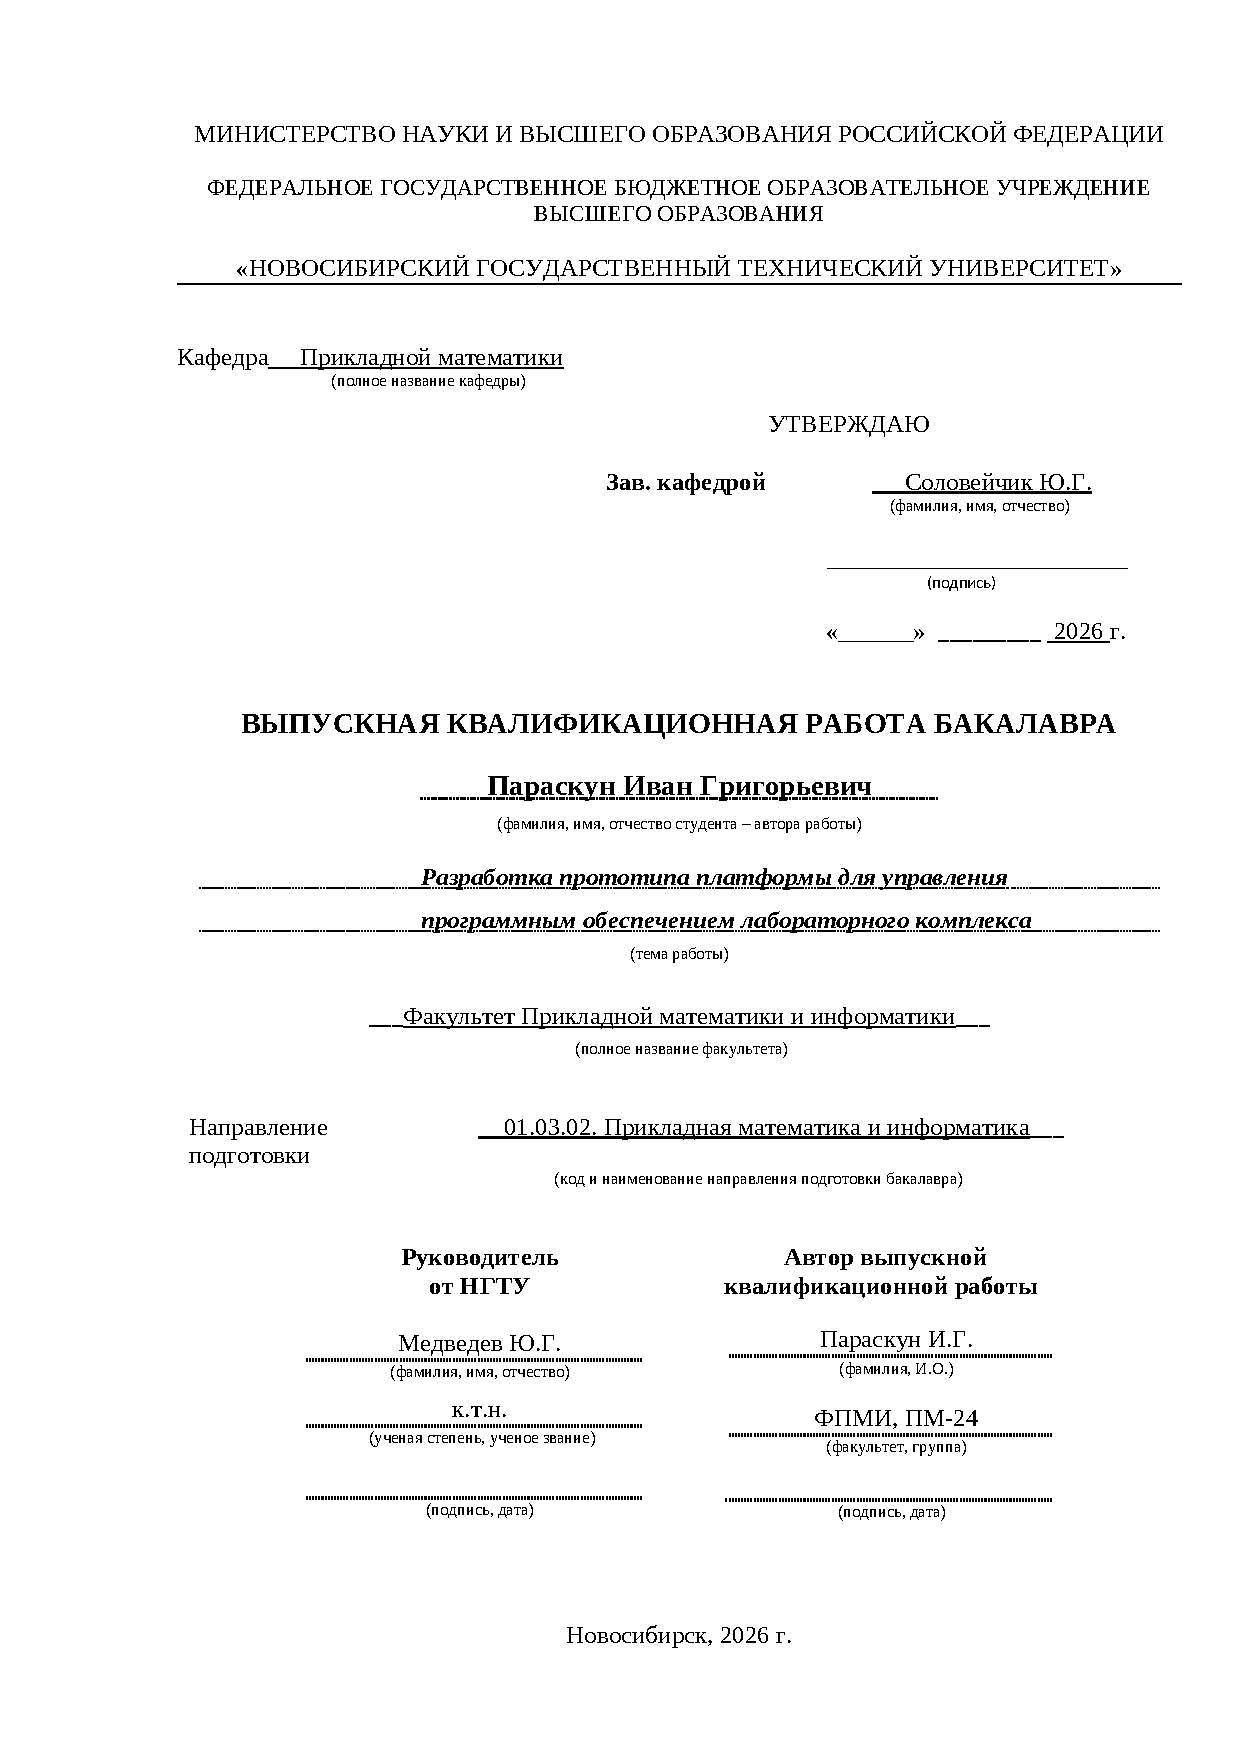
\includepdf{extra/thesis-title.pdf} 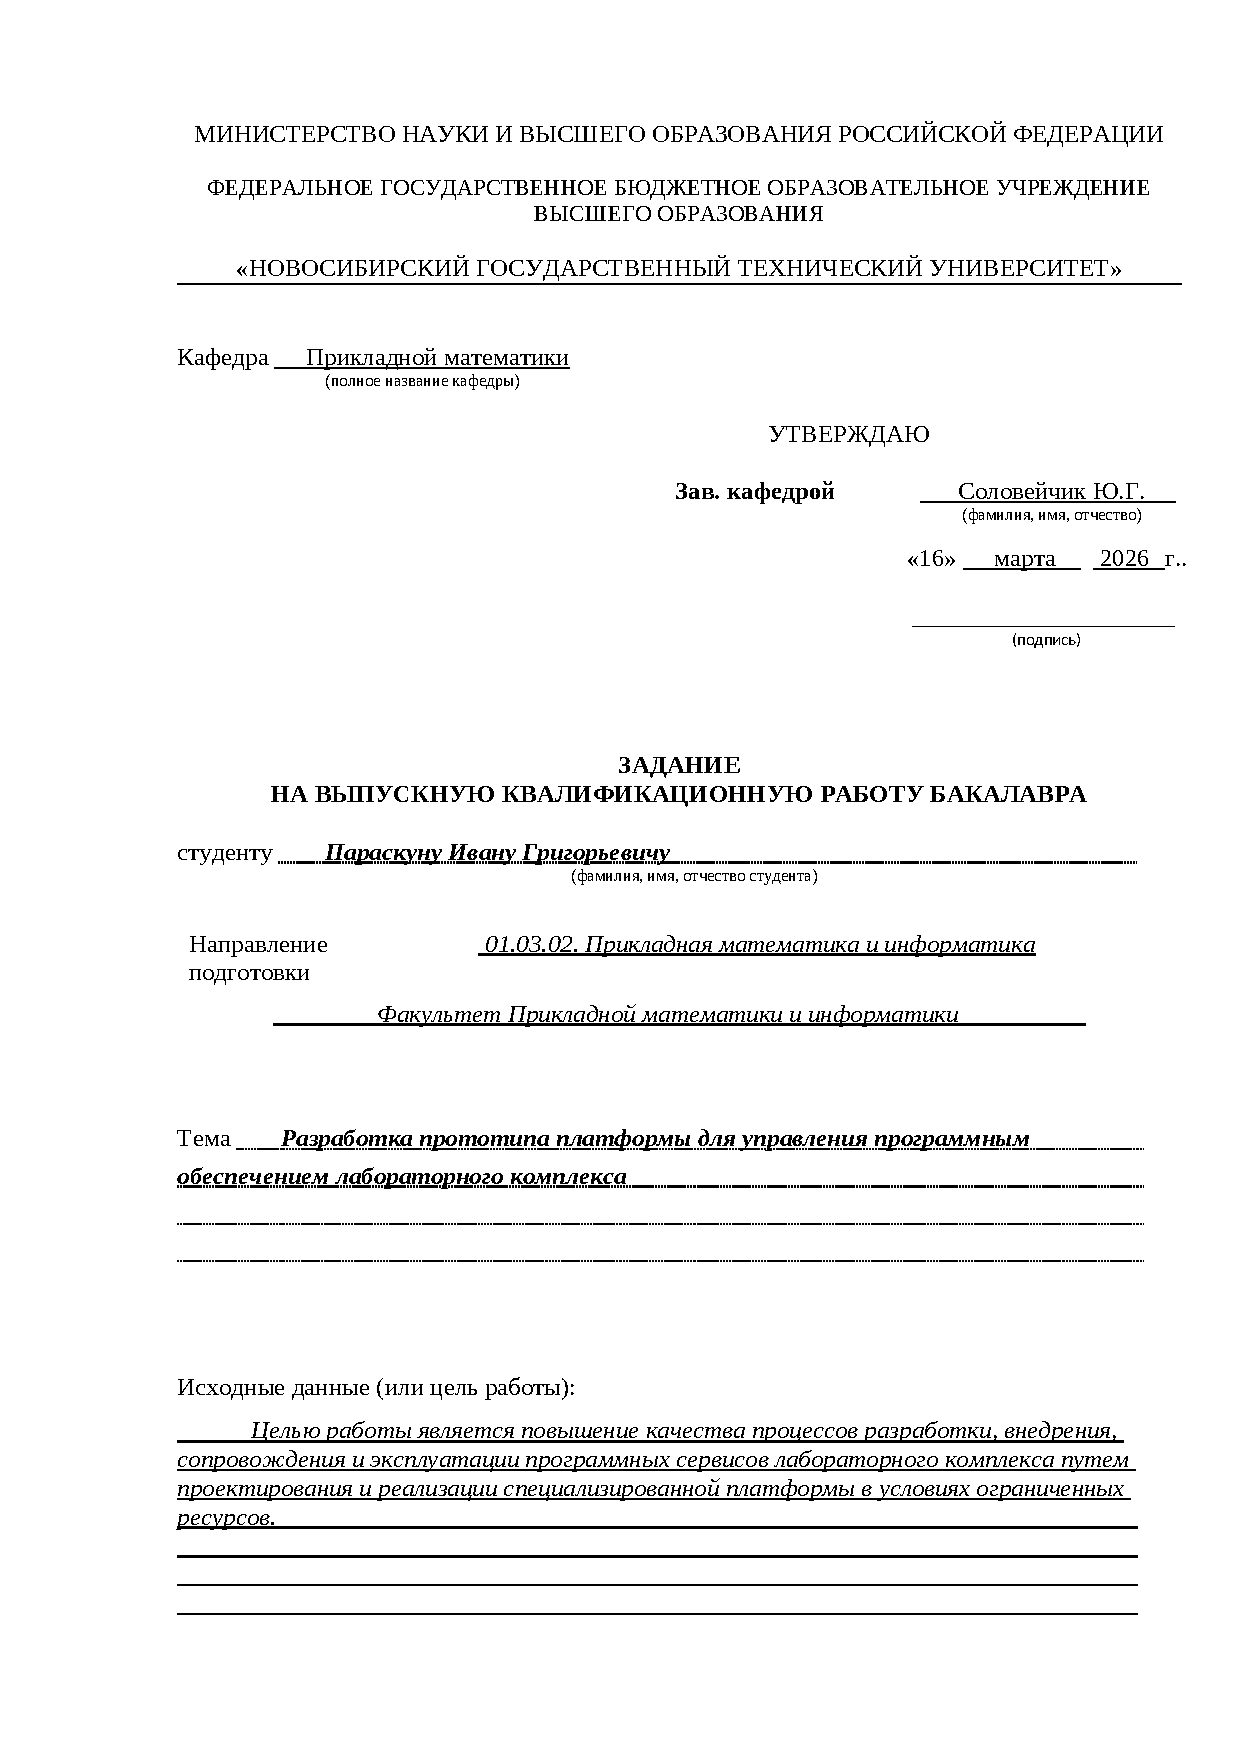
\includepdf[pages=-]{extra/thesis-task.pdf}

	\chapter*{Аннотация}

	Отчет \pageref{LastPage} с., \total{chapter} ч., \total{figure} рис., 0 табл., 10 источников, 3
	прил.

	\bigskip
	ИНСТРУМЕНТЫ РАЗРАБОТКИ, АВТОМАТИЗАЦИЯ, УПРАВЛЕНИЕ,
	\linebreak
	ИНФРАСТРУКТУРА
	\bigskip

	Объект разработки -- проектирование системы.

	Цель работы -- повышение качества процессов разработки, внедрения, сопровождения и эксплуатации
	программных сервисов лабораторного комплекса.

	В результате получена и частично интегрирована система разработки и управления программными
	сервисами лабораторного комплекса.

	\pagenumbering{gobble}
	\renewcommand{\contentsname}{Содержание}
	\tableofcontents
	\newpage
	\pagenumbering{arabic}
	\setcounter{page}{5}

	\addchap{Введение}\subfile{src/intro.tex}

	\chapter{Обзор и постановка задачи}
	\subfile{src/overview.tex}

	\chapter{Концептуальное проектирование}
	\subfile{src/arch.tex}

	\chapter{Реализация}
	\subfile{src/impl.tex}

	\chapter{Верификация}
	\subfile{src/eval.tex}

	\addchap{Заключение} \subfile{src/conclusion.tex}

	\sloppy
	\printbibliography

	\addchap{Приложение А. Менеджер сервисов}\label{apx:1}\subfile{src/apx.sm.tex}

	\addchap{Приложение Б. Потоковый сервис}\label{apx:2}\subfile{src/apx.em-es.tex}

	\addchap{Приложение В. Пакетный сервис}\label{apx:3}\subfile{src/apx.sol.tex}
\end{document}